\documentclass[10pt,a4paper,british]{article}
\usepackage[utf8]{inputenc}
\usepackage{fullpage}
\usepackage{graphicx}
\usepackage{fancyhdr}
\usepackage{comment}
\setlength{\headheight}{13pt}
\pagestyle{fancy}

% default sans-serif
\renewcommand{\familydefault}{\sfdefault}

% floats, caption, etc
\usepackage{occi}

% Highlights
\newcommand{\hl}{\texttt}
%\usepackage{soul}

% no lines for headers and footers
\renewcommand{\headrulewidth}{0pt}
\renewcommand{\footrulewidth}{0pt}

% header
\fancyhf{}
\lhead{GWD-R}
\rhead{\today}

% footer
\lfoot{occi-wg@ogf.org}
\rfoot{\thepage}

% paragraphs need some space...
\setlength{\parindent}{0pt}
\setlength{\parskip}{1ex plus 0.5ex minus 0.2ex}

% some space between header and text...
\headsep 13pt

\setcounter{secnumdepth}{4}

\begin{document}

% header on first page is different
\thispagestyle{empty}

GWD-R \hfill  Thijs Metsch, Platform Computing\\
OCCI-WG \hfill  Andy Edmonds, Intel\\
\rightline {Ralf Nyrén, Aurenav}\\
\rightline {October 14, 2010}\\
\rightline {Updated: \today}

\vspace*{0.5in}

\begin{Large}
\textbf{Open Cloud Computing Interface - Core and Models}
\end{Large}

\vspace*{0.5in}

\underline{Status of this Document}

This document provides information to the community regarding the
specification of the Open Cloud Computing Interface. Distribution is
unlimited.

\underline{Obsoletes}

This document obsoletes GFD-xxx [REFERENCE].

\underline{Copyright Notice}

Copyright \copyright Open Grid Forum (2009-2010). All Rights Reserved.

\underline{Trademarks}

OCCI is a trademark of the Open Grid Forum.

\underline{Abstract}

This document, part of a document series, produced by the OCCI working
group within the Open Grid Forum (OGF), provides a high-level
definition of a Protocol and API. The document is based upon
previously gathered requirements and focuses on the scope of important
capabilities required to support modern service offerings.

\newpage
\tableofcontents
\newpage

\section{Introduction}
The Open Cloud Computing Interface (OCCI) is a RESTful Protocol and
API for all kinds of management tasks. OCCI was originally initiated
to create a remote management API for IaaS%
\footnote{Infrastructure as a Service}
model-based services, allowing for the development of interoperable tools for
common tasks including deployment, autonomic scaling and monitoring.
%
It has since evolved into an flexible API with a strong focus on
interoperability while still offering a high degree of extensibility. The
current release of the Open Cloud Computing Interface is suitable to serve many
other models in addition to IaaS, including e.g.~PaaS and SaaS.

In order to be modular and extensible the current OCCI specification is
released as a suite of complimentary documents, which together form the complete
specification.
%
The documents are divided into three categories consisting of the OCCI Core,
the OCCI Renderings and the OCCI Extensions.
%
\begin{itemize}
\item The OCCI Core specification consists of a single document defining the
 OCCI Core Model. The OCCI Core Model can be interacted with {\em
 renderings} (including associated behaviours) and expanded through {\em extensions}.
\item The OCCI Rendering specifications consist of multiple documents each
 describing a particular rendering of the OCCI Core Model. Multiple renderings can
 interact with the same instance of the OCCI Core Model and will automatically support
 any additions to the model which follow the extension rules defined in OCCI
 Core.
\item The OCCI Extension specifications consist of multiple documents each
 describing a particular extension of the OCCI Core Model. The extension documents
 describe additions to the OCCI Core Model defined within the OCCI specification
 suite.
\end{itemize}
%
The current specification consist of three documents.
Future releases of OCCI may include additional rendering and extension
specifications. The documents of the current OCCI specification suite are:

\begin{description}
\item[OCCI Core] describes the formal definition of the the OCCI Core Model
\cite{occi:core}.
\item[OCCI HTTP Rendering] defines how to interact with the OCCI Core Model using the
RESTful OCCI API \cite{occi:http_rendering}. The document defines how the OCCI Core Model can
be communicated and thus serialised using the HTTP protocol.
\item[OCCI Infrastructure] contains the definition of the OCCI Infrastructure
extension for the IaaS domain \cite{occi:infrastructure}. The document defines
additional resource types, their attributes and the actions that can be taken
on each resource type.
\end{description}


\section{Notational Conventions}
All these parts and the information within are mandatory for
implementors (unless otherwise specified). The key words "MUST", "MUST
NOT", "REQUIRED", "SHALL", "SHALL NOT", "SHOULD", "SHOULD NOT",
"RECOMMENDED", "MAY", and "OPTIONAL" in this document are to be
interpreted as described in RFC 2119 \cite{rfc2119}.

\textbf{Andy: we need to state that this document as part of the current document set,
supersedes all previous documents.}


\section{OCCI model}
OCCI is a boundary protocol and API
that acts as a service front-end to a provider's internal management
framework. Figure~\ref{fig:placement} shows OCCI's place in a
provider's architecture.

\begin{figure}[!hp]
	\centering
	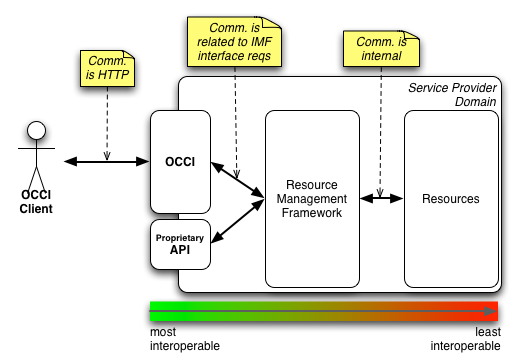
\includegraphics[scale=0.5]{figs/occi-intro.png}
	\caption{OCCI's place in a provider's architecture}
	\label{fig:placement}
\end{figure}

The heart of the OCCI model is the \hl{Resource} type. Any resource exposed
through OCCI is a \hl{Resource} or sub-type thereof.
A resource can be e.g. a virtual machine, a job in a job submission system, a
user, etc.
%
The \hl{Resource} type contains a number of common attributes that
domain-specific \hl{Resource} types inherit. The \hl{Resource} type is
complemented by the \hl{Link} type which associates one \hl{Resource} instance
with another.
%
The \hl{Link} type also contains a number of common attributes that
domain-specific \hl{Link} types inherit.

\hl{Kind} is an abstract type which both \hl{Resource} and \hl{Link} inherit.
Each sub-type of \hl{Kind} is identified by a unique \hl{Type} instance.
%
The \hl{Type} type comprise the classification system built into the OCCI
model. \hl{Type} is a specialisation of \hl{Category} and introduce additional
capabilities in terms of \hl{Action} types.

\begin{figure}[!h]
{\centering \resizebox*{0.9\columnwidth}{!}{\rotatebox{270}
      {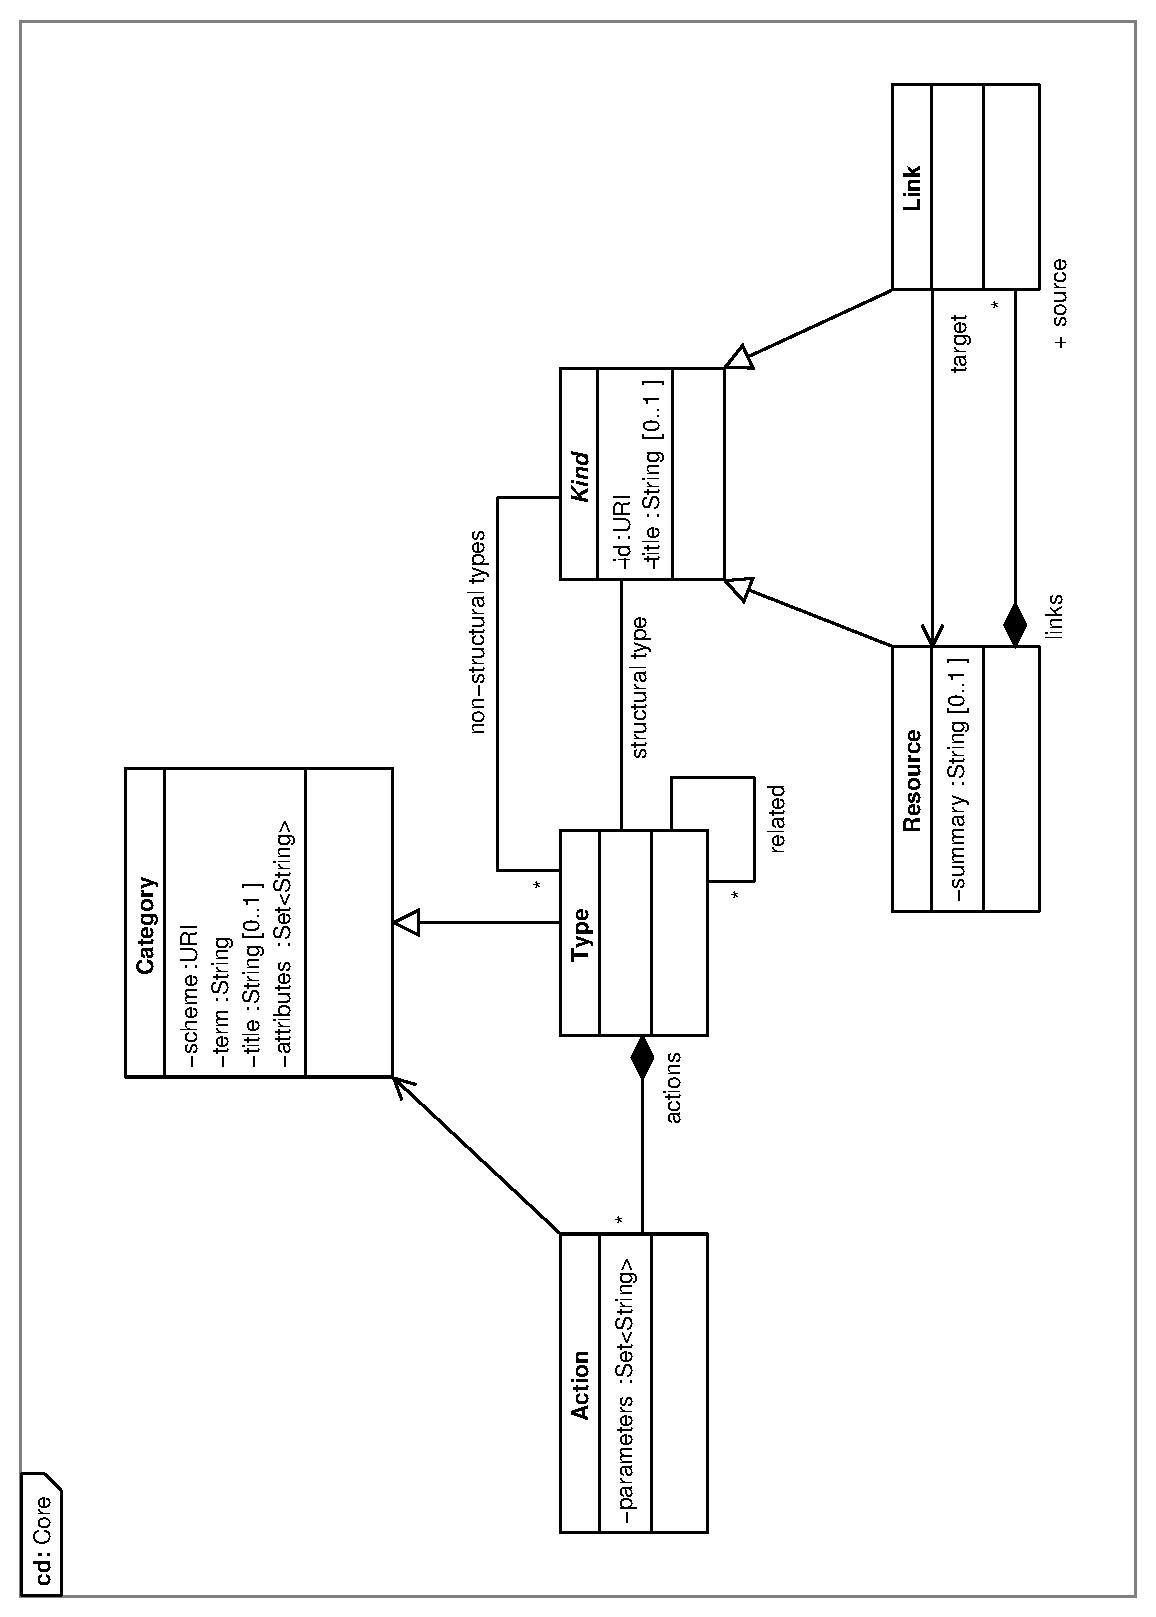
\includegraphics{figs/core_model.pdf}}} \par}
\caption{UML class diagram of the OCCI model. The diagram provides an
overview of the OCCI model but is not a standalone definition thereof}
\label{fig:occi_model}
\end{figure}

The UML class diagram shown in figure~\ref{fig:occi_model} gives an overview of
the OCCI model.  For compliance with OCCI Core, all of the types defined in
the OCCI model MUST be implemented.
The following sections of the specification define the details of the OCCI
model.

\subsection{Classification and Identification}

The OCCI model provides a builtin classification system allowing for safe
extension towards domin-specific usage. This system is like a ``type system''
but with the possiblity of being easily exposed over a text based protocol.
%
The classification system can be summarised with the following key features:
\begin{itemize}
\item Each OCCI base type and extension thereof is assigned a unique
 identifier, a structural \hl{Type}, which allow for dynamic discovery of available
 types.
\item The relationship of structural \hl{Type}s is part of the system and thus
 the inheritance model is also discoverable.
\item The classification system allow non-structural \hl{Type}s to be assigned
 to resource instances adding new capabilities using a mix-in model.
\item Tagging of resource instances is supported through mix-in of
 non-structural \hl{Type}s which have no additional capabilities defined.
\item A collection of associated resources is implicitly defined for each
 structural and non-structural \hl{Type}. I.e.~all resource instances
 associated with a particular \hl{Type} instance form a collection.
\end{itemize}

\subsubsection{Type}

The \hl{Type} type comprise the classification system provided by OCCI
model. It MUST be implemented. A \hl{Type} instance can be either structural or
non-structural.

\mytablefloat{\label{tbl:type}Attributes defined for the \hl{Type} type}{
\begin{tabular}{llllp{2.7in}}
\toprule
Attribute & Type & Multiplicity & Client Mutability & Description \\
\colrule
actions & \hl{Action} & 0..* & Immutable & Set of \hl{Action}s defined by the \hl{Type} instance. \\
related & \hl{Type} & 0..* & Immutable & Set of related \hl{Type} instances. \\
kind & \hl{Kind} & 0..1 & Immutable & \hl{Kind} type uniquely identified by the \hl{Type} instance. \\
\botrule
\end{tabular}
}
The \hl{Type} type inherit the \hl{Category} type and all inherited
attributes MUST be implemented. Table~\ref{tbl:type} defines the
additional attributes the \hl{Type} type MUST implement to be compliant.

\paragraph*{Structural Type}
A structural \hl{Type} is an instance of \hl{Type} assigned as the unique
identifier of a \hl{Kind} sub-type. The following rules apply:
\begin{itemize}
\item A structural \hl{Type} define the capabilities of a \hl{Kind} sub-type in terms of attributes and \hl{Action}s.
\item A unique structural \hl{Type} MUST be assigned to each and every sub-type
 of \hl{Kind}.
\item A structural \hl{Type} MUST be related, either directly or indirectly, to
 the structural \hl{Type} of \hl{Kind},
 i.e.~\textit{http://schemas.ogf.org/occi/core\#kind}.
 %
 See section~\ref{sec:type_relationship} for the definition of \hl{Type}
 relationship.
\item If type {\bf B} inherit type {\bf A}, where {\bf A} is a sub-type of
 \hl{Kind}, the structural \hl{Type} of {\bf B} MUST be directly related to the
 structural \hl{Type} of {\bf A}.
\end{itemize}

\paragraph*{Non-structural Type} A non-structural \hl{Type} is an instance of
\hl{Type} {\em not} assigned as the unique identifier of any \hl{Kind} sub-type.
The following rules apply:
\begin{itemize}
\item A non-structural \hl{Type} define additional capabilities for each
 \hl{Kind} sub-type instance it is associated with. A non-structural \hl{Type}
 add capabilities using a mix-in like model.
\item A non-structural \hl{Type} MUST only be associated with \hl{Kind}
 sub-type {\em instances}, either at creation-time or run-time.
\item A non-structural \hl{Type} MUST NOT be related, neither directly nor
 indirectly, to the structural \hl{Type} of \hl{Kind},
 i.e.~\textit{http://schemas.ogf.org/occi/core\#kind}.
 %
 See section~\ref{sec:type_relationship} for the definition of \hl{Type}
 relationship.
\item A non-structural \hl{Type} defining no additional capabilities in terms
 of attributes or \hl{Action}s is considered to be a tag.
\end{itemize}

\subsubsection{Category}

The \hl{Category} type comprise basis of identification used by the OCCI
classification system. It MUST be implemented. Instances of the \hl{Category}
type are only used to identify \hl{Action} types. All other uses of
\hl{Category} properties are managed through its sub-type \hl{Type}.
%
Table~\ref{tbl:type} defines the attributes the \hl{Category} type MUST
implement to be compliant.

\mytablefloat{\label{tbl:category}Attributes defined for the \hl{Category} type}{
\begin{tabular}{llllp{2.7in}}
\toprule
Attribute & Type & Multiplicity & Client Mutability & Description \\
\colrule
term & String & 1 & Immutable & Unique identifier of the \hl{Category} instance within the categorization scheme. \\
scheme & URI & 1 & Immutable & The categorization scheme. \\
title & String & 0..1 & Immutable & Denotes the display name of an instance. \\
attributes & String & 0..* & Immutable & Comprise the resource attribute names defined by the \hl{Category} instance. \\
\botrule
\end{tabular}
}

A \hl{Category} is uniquely identified by concatenating the categorization
scheme with the category term,
e.g.~\textit{http://example.com/category/scheme\#term}.
This is done to enable discovery of \hl{Category} definitions in text based
renderings such as HTTP. All renderings MUST make use and understand
concatenated unique identifiers of \hl{Category} types.
%
Sub-types of \hl{Category} such as \hl{Type} inherit this property.

The categorization schemes defined in the OCCI specification all use the
\textit{http://schemas.ogf.org/occi/} base URL. This base URL is reserved for
OCCI an MUST NOT be used by domain-specific extensions.

Attribute names defined by \hl{Category} instances%
\footnote{Also applies to \hl{Type} instances.}
use the \texttt{occi.}~prefix.  This prefix is reserved for OCCI and MUST NOT
be used by domain-specific extensions.

\subsubsection{Type relationship}
\label{sec:type_relationship}
As previously defined a structural \hl{Type} MUST be related, either
either directly or indirectly, to the structural \hl{Type} of \hl{Kind},
i.e.~\textit{http://schemas.ogf.org/occi/core\#kind}.
%
The OCCI base types \hl{Resource} and \hl{Link} extending \hl{Kind}, and any
futher sub-typing, implies a hierarchy of related structural \hl{Type}
instances. This \hl{Type} relationship thus mirror the type inheritance
structure of the OCCI model and any extension thereof.

In an example where a domain-specific ``Custom Compute Resource'' is a sub-type
the OCCI infrastructure type Compute, which in turn is a sub-type of the
\hl{Resource} type, four related structural \hl{Type}s would be involved.
%
Table~\ref{tbl:relationship} illustrates the exemplified hierarchy of \hl{Type}
instances relating the domain-specific structural \hl{Type} to the structural
\hl{Type} of \hl{Kind}.

\mytablefloat{\label{tbl:relationship}Exempel of the \hl{Type} relationship involved
for a domain-specific extension of the OCCI infrastructure type \hl{Compute}.}{
\begin{tabular}{p{7cm}p{7cm}}
\toprule
Structural Type & Related Structural Type \\
\colrule
\textit{http://example.com/occi/custom\#compute} & \textit{http://schemas.ogf.org/occi/infrastructure\#compute} \\
\textit{http://schemas.ogf.org/occi/infrastructure\#compute} & \textit{http://schemas.ogf.org/occi/core\#resource} \\
\textit{http://schemas.ogf.org/occi/core\#resource} & \textit{http://schemas.ogf.org/occi/core\#kind} \\
\botrule
\end{tabular}
}

\subsubsection{Type assignment}
\label{sec:type_assignment}
A structural \hl{Type} MUST be statically assigned to each sub-type of
\hl{Kind} defined by an implementation. A \hl{Kind} sub-type instance MUST be
automatically associated with its structural \hl{Type} at creation-time.  The
structural \hl{Type} associated with an instance MUST remain associated with the
instance during its lifetime.

A non-structural \hl{Type}, also known as a mix-in, MAY be associated with a
\hl{Kind} sub-type instance, either at creation-time or run-time. An OCCI
implementation MAY restrict which instances can be associated with a particular
non-structural \hl{Type}.

\subsubsection{Collections}
\label{sec:collection}
One or more \hl{Kind} sub-type instances associated with the same \hl{Type},
may it be structural or non-structural, automatically form a collection.
Each \hl{Type} instance in the system identifies a collection consisting of all
different \hl{Kind} sub-type instances associated with the \hl{Type}.

A \hl{Kind} sub-type instance is always a member of the \hl{Kind}'s structural
\hl{Type} collection since a \hl{Kind} sub-type instance MUST be associated
with the structural \hl{Type} of the \hl{Kind} sub-type.
Since a non-structural \hl{Type} can be assigned to any \hl{Kind} sub-type
instance a collection can contain instances of different \hl{Kind} sub-types.

For example an instance of the \hl{Resource} type will always be associated
with the \textit{http://scheme.ogf.org/occi/core\#resource} \hl{Type} and thus
part of the \hl{Resource} \hl{Type} collection.

\subsubsection{Discovery}
\label{sec:discovery}
An OCCI client MUST be able to discover all instances of \hl{Type} and
\hl{Category} a particular service provider's OCCI implementation support. By
examining these instances a client MUST be able to, at a minimum, deduce the
following information:
\begin{itemize}
\item The \hl{Kind} sub-types available from a the service provider, including domain-specific extensions.
\item The attributes associated with each \hl{Kind} sub-type.
\item The invocable operations, i.e. \hl{Action}s, defined for each \hl{Kind} sub-type.
\item Additional mix-ins or tags, i.e. non-structural \hl{Type}s, applicable to
 \hl{Kind} sub-type instances.
\end{itemize}
The above requirements comprise the OCCI discovery mechanism. It MUST be
implemented.
%
The details of exactly how the \hl{Category} and \hl{Type} instances are
exposed to an OCCI client is specific to the particular rendering used.
\marginpar{References?}
The relevant details can be found in the OCCI rendering documents.

%%%%%%%%%%%%%%%%%%%%%%%%%%%%% Bits and pieces %%%%%%%%%%%%%%%%%%%%%%%%%%%%%%%%%%

% Stuff which may or may not be useful to add somewhere in the spec...

\begin{comment}
The central component of the classification system is the \hl{Type} type which
is a specialisation of the \hl{Category} type. The following sections describe
the OCCI classification system in detail.

Each OCCI base type, see section~\ref{sec:base_types}, is assigned a
unique identifier.  This identifier is an instance of \hl{Type} and comprise
the structural \hl{Type} of the associated base type%
\footnote{The \hl{Action} type is an exception and is instead uniquely
identified by a \hl{Category} instance. An \hl{Action} is a capability of \hl{Type}
and can therefore not be identified by \hl{Type}.}.
\end{comment}


\begin{comment}
%%% CLIENT Interaction, do we need to specify this explicitly?!
\subsubsection{Creating Instances}
A client MUST supply the concrete Kind type as a Category. All OCCI
implementations MUST understand these requests containing concrete
Kind types, i.e. Resource, Link, Action or a subtype thereof.

When a client attempts to add a non-structural
\hl{Type} at a stage not supported by a particular provider's OCCI
implementation, the provider MUST notify the client it has issued a bad
request.
\end{comment}

%%%%%%%%%%%%%%%%%%%%%%%%%%%%%%%%%%%%%%%%%%%%%%%%%%%%%%%%%%%%%%%%%%%%%%%%%%%%%%%


\subsection{The OCCI base types}
\label{sec:base_types}
The following sections describe the base types of the OCCI core
model. The base types are Kind, Category, Resource, Link and
Action. All base types MUST be implemented.

\subsubsection{Kind}
The Kind type is an abstract base type and common to all resources in
the OCCI context. It MUST be implemented. Kind enforces for all
subtypes a required id attribute and an (optional) title
attribute. More importantly Kind introduces one or more type mix-ins
through the type Category (see section \ref{sec:type_system}). The
following table defines the attributes the Kind type MUST implement to
be compliant:

\begin{tabular}{l|l|l|l|p{2.7in}}
Attribute & Type & Multiplicity & Client Mutability & Description \\
\hline
id & URI & 1 & Immutable & Denotes a unique (within the service provider's name-space) identifier of a Kind subtype instance. \\
title & String & 0..1 & Mutable & Denotes the display name of an instance. \\
categories & Category & 1..* & Mutable\footnotemark[1] & Comprises the Category types associated to this instance. Consumers can expect the attributes and actions of the associated Category types to be exposed by the instance. \\ 
\end{tabular}
\footnotetext[1]{Only tag Category types are client mutable.}
\addtocounter{footnote}{1}

\subsubsection{Category}
The Category type represent the classification mechanism used by
OCCI. It MUST be implemented. From a system point of view a Category
is used for two different classification purposes. See also section
\ref{sec:type_system} ``Type System'' and section \ref{sec:collection}
``Collections''.

\begin{description}
\item[Taxonomy] A Category is used to assign static type information
  to each resource type inheriting Kind or a descendant of Kind. This
  use of Category types denotes the OCCI "static type system". A
  unique Category MUST be assigned to every descendant of Kind. See
  the section \ref{sec:hierarchy} "Hierarchy".
\item[Folksonomy] A Category can be used to assign tags to resource
  instances via a mix-in like model. A Category mix-in MUST NOT be
  related to an OCCI base type (or any descendant of Kind) and MUST
  NOT be the unique identifier thereof.  Example use cases are
  collections, location information and templates for virtual machine
  provisioning.
\end{description}

The following table defines the attributes the Category type MUST
implement to be compliant:

\begin{tabular}{l|l|l|l|p{2.7in}}
Attribute & Type & Multiplicity & Client Mutability & Description \\
\hline
term & String & 1 & Immutable & The category to which the resource belongs. \\
scheme & URI & 1 & Immutable & The categorization scheme. \\
title & String & 0..1 & Immutable & Denotes the display name of an instance. \\
attributes & String & 0..* & Immutable & Comprise the resource attributes defined by the Category. \\
related & Category & 0..* & Immutable & Set of related Category types. \\
\end{tabular}

A Category is uniquely identified by concatenating the categorization
scheme with the category term,
e.g. \textit{http://example.com/category/scheme\#term}.  This is done
to enable discovery of Category definitions per HTTP. All renderings
MUST make use and understand concatenated unique identifiers of
Category types.

\paragraph{Hierarchy}
\label{sec:hierarchy}
To be a part of the "static type system" a Category MUST be related,
either directly or indirectly, to a base type Category. Extension of
the OCCI base types through subtyping thus implies a hierarchy of
related Category types.

In an example where "Custom-Compute-Resource" is a subtype of
"Compute-Resource", which in turn is a subtype of the Resource base
type, three related Category types would be involved. The following
table illustrates the exemplified hierarchy of Category types relating
the custom Category to a base type Category.

Example:

\begin{tabular}{p{0.6in}|p{3.1in}|p{2in}}
Kind & Category & Related Category \\
\hline
Custom-Compute-Resource & \textit{http://example.com/occi/custom\#compute} & \textit{http://schemas.ogf.org/occi/infrastructure\#compute} \\
Compute-Resource & \textit{http://schemas.ogf.org/occi/infrastructure\#compute} & \textit{http://schemas.ogf.org/occi/core\#resource} \\
Resource & \textit{http://schemas.ogf.org/occi/core\#resource} & none \\
\end{tabular}

\subsubsection{Resource}
The Resource type describes a concrete resource that can be inspected
and manipulated. It represents a general object in the OCCI core model
and MUST be implemented. Resource enforces the inheritance of a set of
common attributes into subtypes (such as a unique identifier and an
optional descriptive summary). Moreover, it introduces relationships
to other Resource instances, denoted by Links. It also introduces
operations that can be invoked on this instance, denoted by Actions.

The Resource type is assigned the
\textit{http://schemas.ogf.org/occi/core\#resource} Category.

\begin{itemize}
  \item A Resource instance MUST at least expose this or a related
    Category together with any associated attributes.
  \item A Resource instance MUST advertise those of its Actions, if
    any, which are currently applicable.
  \item A Resource instance MUST implement the attributes in the
    following table:
\end{itemize}

\begin{tabular}{l|l|l|l|p{2.7in}}
Attribute & Type & Multiplicity & Client Mutability & Description \\
\hline
summary & String & 0..1 & Mutable & Holds a summarizing description of the Resource instance.\\
links & Link & 0..* & Mutable & Comprises a set of Link compositions. Being a composite relation the removal of a Link from the set MUST also remove the Link instance.\\
actions & Action & 0..* & Immutable & Set of Actions associated with the Resource.\\
\end{tabular}

The OCCI Extension documents define sets of specific subtypes of
Resources, Links and Actions. They inherit Resource and is each
assigned an unique Category.

\subsubsection{Link}
The Link type defines a base association between two Resources. It
MUST be implemented. Link indicates that one resource is connected to
another.

The Link type is assigned the
\textit{http://schemas.ogf.org/occi/core\#link Category}. A Link
instance MUST at least expose this or a related Category together with
any associated attributes. A Link instance MUST also implement the
attributes in the following table:

\begin{tabular}{l|l|l|l|p{2.7in}}
Attribute & Type & Multiplicity & Client Mutability & Description \\
\hline
source & Resource & 1 & Mutable & Denotes the resource the Link instance originates from.\\
target & Resource & 1 & Mutable & Denotes the resource the Link instance points to.\\
\end{tabular}

The Link base type MUST NOT refer to an external resource. A provider
MAY however create a subtype of Link with different semantics that
e.g. have a target attribute containing an URI and thus the ability of
linking with external resources.

\subsubsection{Action}
The Action type defines an invocable operation on an associated
Resource. It MUST be implemented. In general, Actions modify state
(e.g. by performing a complex operation such as rebooting a virtual
machine).

The Action type is assigned the
\textit{http://schemas.ogf.org/occi/core\#action} Category. An Action
instance MUST at least expose this or a related Category together with
any associated attributes.

\subsection{Mutability}
\marginpar{Does 'client access' need to be discussed here?}
Attributes of a OCCI base type instance, a resource instance, are
either client mutable or client immutable. If an attribute is noted to
be mutable this MUST be interpreted that a client can create a
resource instance that is parametrized by the attribute. Likewise, if
an attribute is mutable, a client can update that resource instance's
mutable attribute value and the server side MUST support this. If an
attribute is marked as immutable, it indicates that the server side
implementation MUST manage these exclusively. Immutable attributes
MUST NOT be modifiable by clients under any circumstance.

\subsection{Type System}
\label{sec:type_system}
The Category type is the classification mechanism used by OCCI. This
tells service providers what type of concrete OCCI Kind should be
created. Each domain-specific section of the OCCI specification
(e.g. infrastructure) defines its own concrete Resource, Action and
optionally Link specializations. It should be noted that depending on
a client's credentials, access to creating certain OCCI Kind sub-type instances
MAY be restricted.

The type system is a flexible and extensible one allowing for the
addition of "mix-in" Category types. Mix-in Category types are ones
that add additional behavior to OCCI Kinds and are Category types not
defined by the OCCI specifications. The mix-in Category types can be
added to an OCCI Kind both at Kind creation-time and run-time. The
Kinds to which a particular mix-in Category type can be applied, is
defined by the provider implementation. At which time, creation- or
run-time, these mix-in types can be applied is also defined by the
provider implementation. Discovery of mix-in types can be achieved by
querying the OCCI Query interface. Mix-in Category types are those
that are NOT related to an OCCI base type Category and MUST be
implemented as such. When a client attempts to add a mix-in at a stage
not supported by the provider, the provider MUST notify the client
that it has issued a bad request.

\subsubsection{Creating Instances}
A client MUST supply the concrete Kind type as a Category. All OCCI
implementations MUST understand these requests containing concrete
Kind types, i.e. Resource, Link, Action or a subtype thereof.

\subsection{Collections}
\label{sec:collection}
One or more Kind sub-type instances assigned to the same Category
automatically form a collection. Each Category in the system
identifies a collection consisting of all different Kind sub-type instances
associated with the Category.

A Kind sub-type instance is always a member of the Kind's identifying
Category collection since a Kind sub-type instance MUST be assigned the
identifying Category of the Kind sub-type.
Since a tag Category can be assigned to any Kind sub-type
instance a collection can contain instances of different Kind
sub-types.

For example an instance of the Resource type will be assigned the
\textit{http://scheme.ogf.org/occi/core\#resource} Category and thus
part of the Resource Category collection.

\subsection{Extensibility}
The OCCI Core model has a flexible yet fairly simple extension
mechanism through the use of sub-typing and Category types.

\subsubsection{Sub-types and Category Types}
The OCCI Core model has a flexible yet fairly simple extension
mechanism through the use of sub-typing and Category types.  A
provider MAY extend the OCCI core model by creating a subtype of
either an OCCI Core base type or a provider defined subtype.

A provider MUST assign a new unique Category to each new subtype
defined. The new Category MUST be, either directly or indirectly,
related to one of the Core base types, i.e. Resource, Link or
Action. If a provider extends a subtype the new Category SHOULD be
related to the subtype extended, provided the previous rule holds
true.

Providers MAY also define new Category types for tagging and
templating purposes. Such a Category MUST NOT be the unique identifier
of a resource type, i.e. must not be part of the "static type system".

The scheme of provider-defined Category types MUST reside in a unique
namespace different from those in the OCCI specification. Any
attributes defined by a new Category MUST NOT have a name starting
with occi. The occi namespace prefix is reserved for extensions which
are standardized. A provider SHOULD use an attribute namespace
comprising the reverse domain name as prefix to every attribute name.

A provider-defined Category identifying a custom subtype of Resource
could be exemplified as follows. The term and scheme is defined by the
provider. The related set MUST include a, direct or indirect (through
a hierarchy), reference to the Resource base type category.

\begin{itemize}
\item term = custom\_resource.
\item scheme = \textit{http://example.com/occi/resource\#}
\item related = \textit{http://schemas.ogf.org/occi/core\#resource}
\end{itemize}

\subsubsection{Extension of the base types}
A provider MAY define subtypes of the Core base types Resource, Link
and Action for domain-specific purposes. A unique Category MUST be
assigned to each new subtype. The assigned Category MUST be directly
related to the Category of the base type extended.

\subsubsection{Extension of subtypes}
A provider MAY define subtypes of any existing subtype, either defined
in OCCI or by someone else. A unique Category MUST be assigned to each
new subtype. The assigned Category MUST be either directly or
indirectly related to a base type Category. It is RECOMMENDED the
Category is related to the Category of the subtype extended.

\subsection{Discovery}
An OCCI client MUST be able to discover all Category types a
particular provider supports before interacting with the
provider. Since the rendering of the Category types is depended of the
protocol the rendering documents give more information on how
information is send and can be parsed.

\section{Contributors}
Editors: Andy Edmonds, Thijs Metsch \\
Contributors: Alexander Papaspyrou, Ralf Nyrén, Sam Johnston

\textbf{TBD: Bunch op people missing here - create table\ldots}

\section{Glossary}
\label{sec:glossary}
\begin{tabular}{l|p{12cm}}
Term & Description \\
\hline
\hl{Action} & An OCCI base type. Represent an invocable operation on a \hl{Entity} sub-type instance or collection thereof. \\

\hl{Category} & A type in the OCCI model. The parent type of \hl{Kind}. \\

\hl{Client} & An OCCI client.\\

\hl{Collection} & A set of \hl{Entity} sub-type instances all associated to a particular \hl{Kind} or \hl{Mixin} instance. \\

\hl{Entity} & An OCCI base type. The parent type of \hl{Resource} and \hl{Link}. \\

\hl{Kind} & A type in the OCCI model. A core component of the OCCI classification system. \\

\hl{Link} & An OCCI base type. A \hl{Link} instance associate one \hl{Resource} instance with another. \\

mixin & An instance of the \hl{Mixin} type associated with a {\bf resource
 instance}. The ``mixin'' concept as used by OCCI {\em only} applies to
 instances, never to \hl{Entity} types. \\

\hl{Mixin} & A type in the OCCI model. A core component of the OCCI classification system. \\

\hl{OCCI} & Open Cloud Computing Interface \\

OCCI base type & One of \hl{Entity}, \hl{Resource}, \hl{Link} or \hl{Action}. \\

OGF & Open Grid Forum \\

\hl{Resource} & An OCCI base type. The parent type for all domain-specific resource types. \\

resource instance & An instance of a sub-type of \hl{Entity}. The OCCI
 model defines two sub-types of \hl{Entity}, the \hl{Resource} type and the
 \hl{Link} type. However, the term {\em resource instance} is defined to
 include any instance of a {\em sub-type} of \hl{Resource} or \hl{Link} as
 well. \\

Tag & A \hl{Mixin} instance with no attributes or actions defined. \\

Template & A \hl{Mixin} instance which if associated at resource instantiation
time pre-populate certain attributes. \\

type & One of the types defined by the OCCI model.  The OCCI model types are
 \hl{Category}, \hl{Kind}, \hl{Mixin}, \hl{Action}, \hl{Entity}, \hl{Resource}
 and \hl{Link}. \\

URI & Uniform Resource Identifier \\
URL & Uniform Resource Locator \\
URN & Uniform Resource Name \\
\end{tabular}



\section{Intellectual Property Statement}
The OGF takes no position regarding the validity or scope of any
intellectual property or other rights that might be claimed to pertain
to the implementation or use of the technology described in this
document or the extent to which any license under such rights might or
might not be available; neither does it represent that it has made any
effort to identify any such rights. Copies of claims of rights made
available for publication and any assurances of licenses to be made
available, or the result of an attempt made to obtain a general
license or permission for the use of such proprietary rights by
implementers or users of this specification can be obtained from the
OGF Secretariat.

The OGF invites any interested party to bring to its attention any
copyrights, patents or patent applications, or other proprietary
rights which may cover technology that may be required to practice
this recommendation. Please address the information to the OGF
Executive Director.


\section{Disclaimer}
This document and the information contained herein is provided on an
``As Is'' basis and the OGF disclaims all warranties, express or
implied, including but not limited to any warranty that the use of the
information herein will not infringe any rights or any implied
warranties of merchantability or fitness for a particular purpose.


\section{Full Copyright Notice}
Copyright \copyright ~Open Grid Forum (2009-2014). All Rights Reserved.

This document and translations of it may be copied and furnished to
others, and derivative works that comment on or otherwise explain it
or assist in its implementation may be prepared, copied, published and
distributed, in whole or in part, without restriction of any kind,
provided that the above copyright notice and this paragraph are
included on all such copies and derivative works. However, this
document itself may not be modified in any way, such as by removing
the copyright notice or references to the OGF or other organizations,
except as needed for the purpose of developing Grid Recommendations in
which case the procedures for copyrights defined in the OGF Document
process must be followed, or as required to translate it into
languages other than English.

The limited permissions granted above are perpetual and will not be
revoked by the OGF or its successors or assignees.


\section{References}

Note that only permanent documents should be cited as
references. Other items, such as Web pages or working groups, should
be cited inline (i.e., see the Open Grid Forum,
http://www.ogf.org). References should conform to a standard such as
used by IEEE/ACM, MLA, Chicago or similar. Include an author, year,
title, publisher, place of publication. For online materials, also add
a URL. It is acceptable to separate out ''normative references,'' as
IETF documents typically do. Some sample citations:

\end{document}
